%%%%%%%%%%%%%%%%%%%%%%%%%%%%%%%%%%%%%%%%%%%%%%%%%%%%%%%%%%%%%%%%%%%%%%%%
% 1. はじめに
%%%%%%%%%%%%%%%%%%%%%%%%%%%%%%%%%%%%%%%%%%%%%%%%%%%%%%%%%%%%%%%%%%%%%%%%
\section{Introduction}
Due to the impact of the COVID-19, it is becoming more important to avoid the crowded places. Trains, buses, restaurants, and elevators tend to be crowded with people. Efforts are being actively made to visualize the congestion in these places and to prevent people from being led to the congested places. In this paper, we focus on the visualization of the congestion level of elevators. The fact that elevators are places where people tend to be crowded is mentioned in a poster by the Ministry of Health, Labor and Welfare of Japan to prevent the spread of the COVID-19\cite{ministry}. The elevator is very narrow and easily crowded. Also, it is difficult for elevator users to avoid congestion. Even if the elevator is not crowded at the time when the user gets on, if many people get on at the intermediate floor, the user who was originally on the elevator will not get off unless the floor is the destination floor. In the opposite pattern, if a user presses the elevator button and waits for the elevator, but the elevator is crowded, the user may give up and wait for the next elevator or be forced to get on. This is considered to be an incident that occurs because the user cannot grasp the status of each floor and the number of people in the elevator at the timing when the elevator button is pressed. If there are users on each floor as described above, the elevator will stop at each floor, which will lead to deterioration of the transportation efficiency of the elevator and increase of the waiting time.


% 図:システム概要
% TODO: 図中の説明は、英語のものに変更する
\begin{figure}[t]
  \begin{center}
    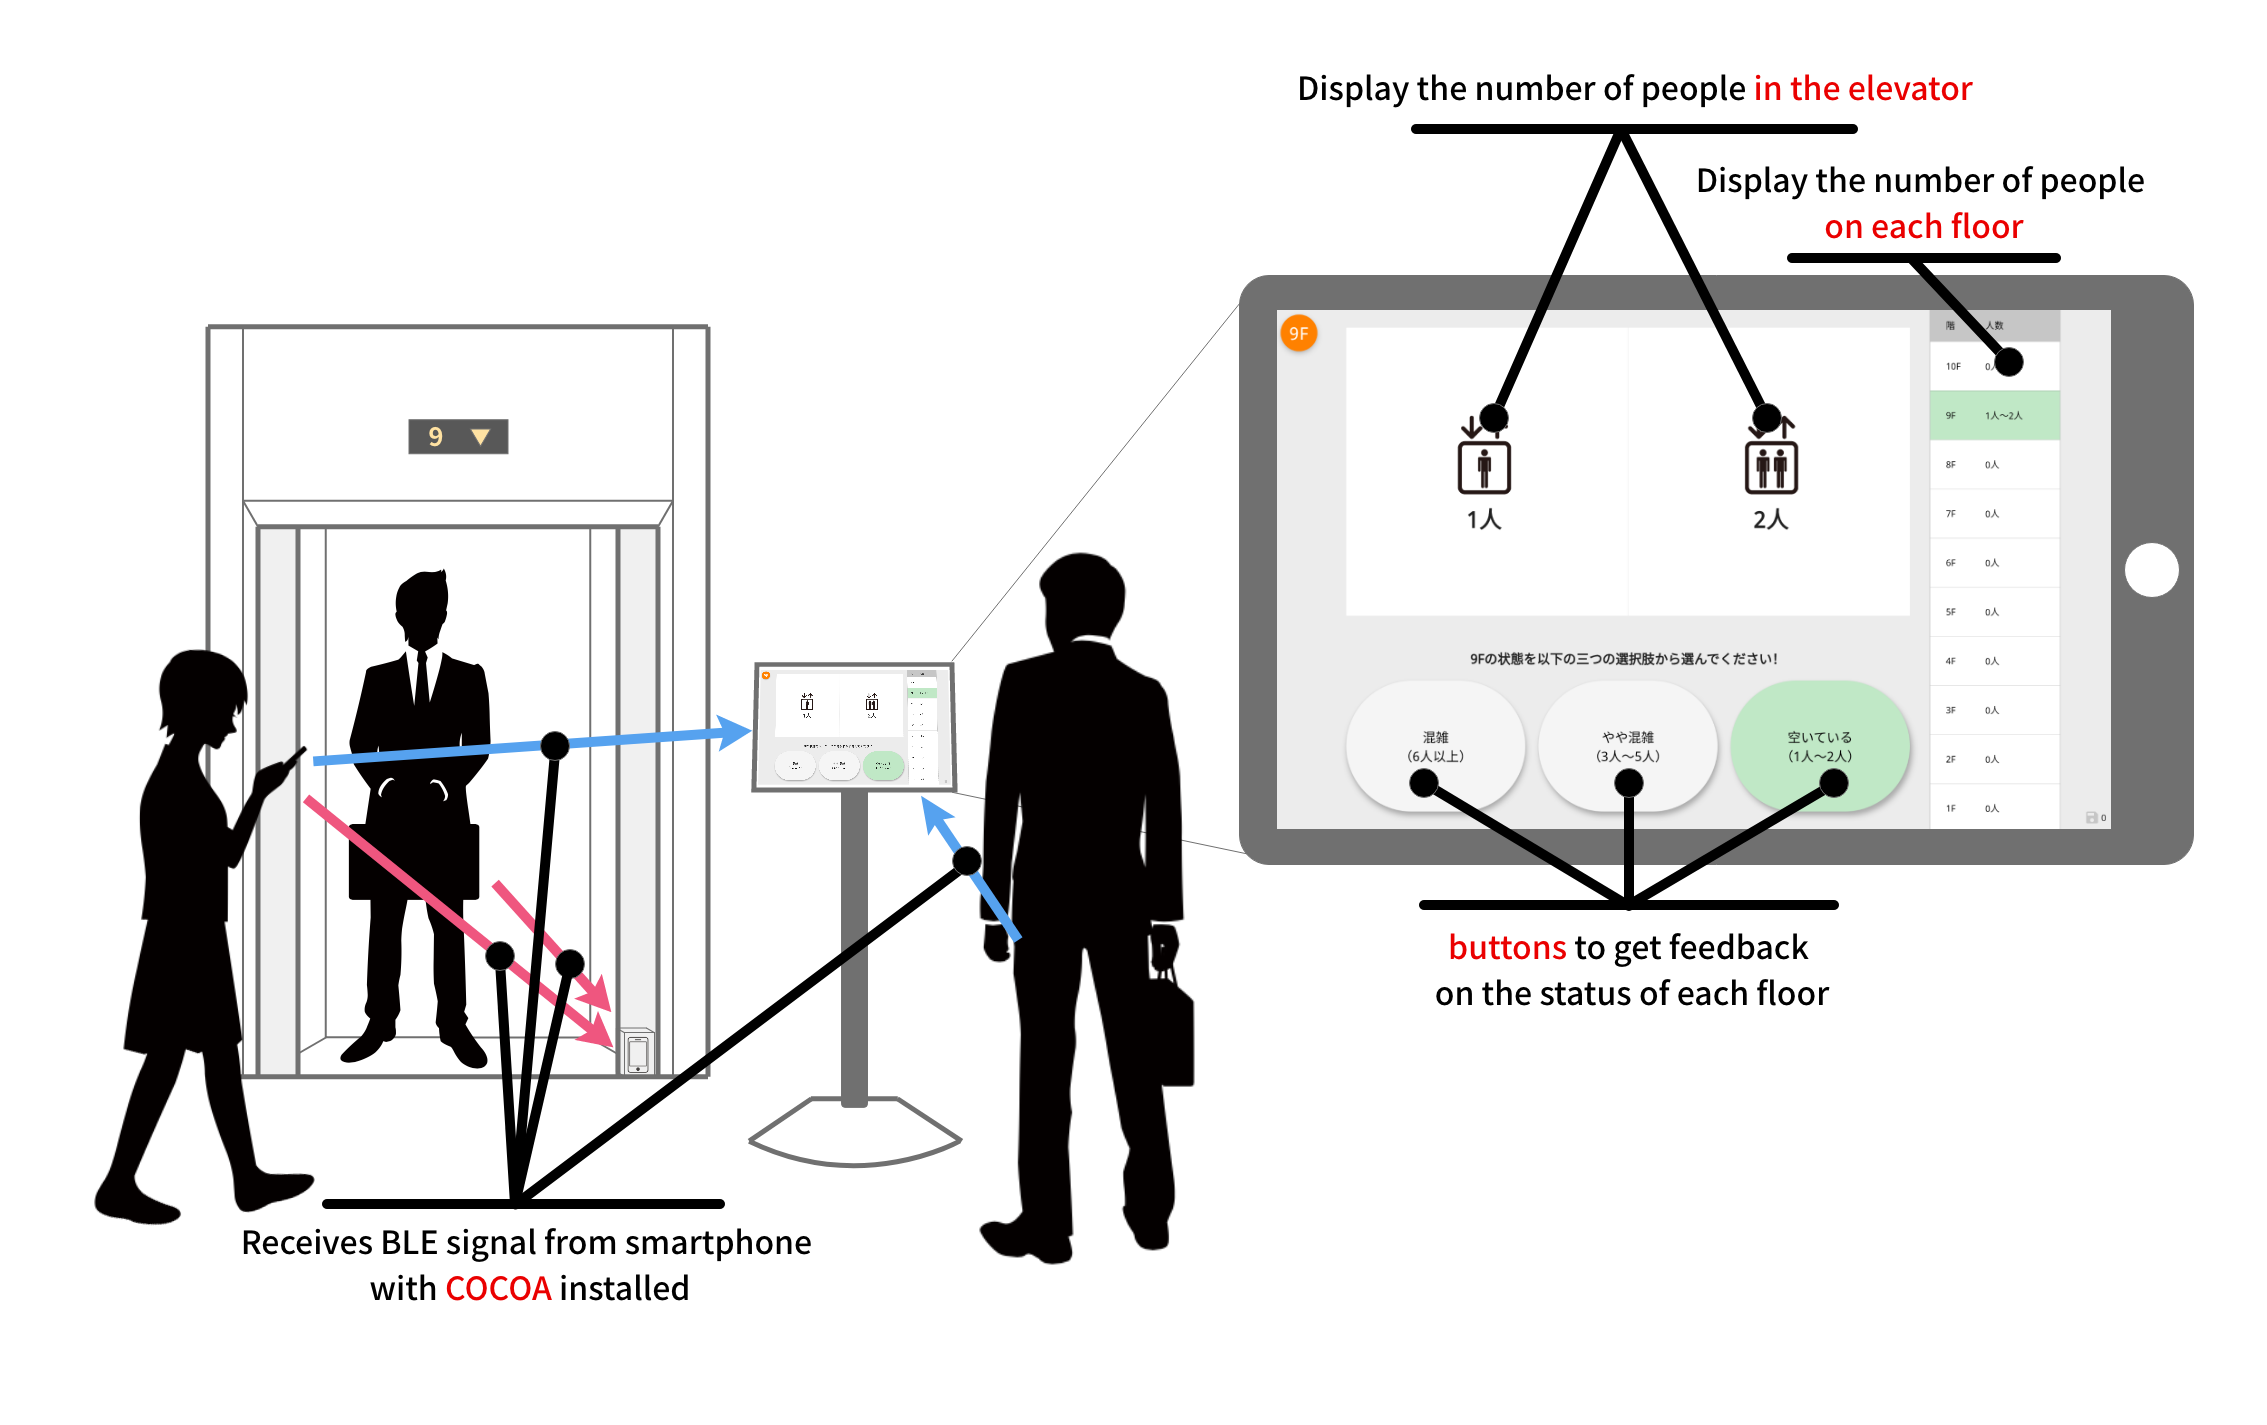
\includegraphics[clip, width=1.0\hsize]{img/system.png}
    \caption{System Overview}
    \label{fig:system}
  \end{center}
\end{figure}


To solve these problems, a method of informing users of the congestion status of elevators through a smartphone application has been proposed by building company, kajima\cite{kajima}. The method using a smartphone application requires the user to install an application, which raises the hurdle to grasp the congestion information. In addition, kajima\cite{kajima} proposes a method for detecting passengers by using a camera as a method to grasp the congestion status in an elevator.
Although the camera-based detection is highly accurate, there are some problems in terms of installation cost, such as privacy issues and the need to install a ceiling. In another approach, a gate is installed in front of the elevator and an ID card is scanned to allow the system to know the number of elevator users and their destinations, and to select the optimal elevator and timing for boarding\cite{elenavi}. Since the number of elevator users is controlled by the gate, it is easy to control the number of elevator users and to eliminate the congestion in the elevators.

% MARK: don't show footnote
\thispagestyle{guusuu}

In this study, we propose a appendable system in which a tablet terminal is installed in front of the elevator to present the number of people in the elevator, the congestion status of each floor (Figure \ref{fig:system}). We believe that this system will solve the problem of not being able to grasp the status of other floors and the number of people in the elevator at the time when the elevator button is pressed, which is a problem unique to elevators. Compared with the method of having users install an application, this system allows users to easily obtain information on congestion, and thus encourages them to make decisions such as using the stairs or waiting for the next elevator before pressing the elevator button.

As a part of the basic experiment, we also evaluated the continuous operation time and detection accuracy of the system, and estimated the behavior pattern and waiting time of the elevator users based on the RSSI time series data of BLE signals acquired from the system.

This paper is organized as follows. In Chapter 2, related research is described, and in Chapter 3, the outline and requirements of the elevator usage visualization system are described. In Chapter 4, the estimation of the user's behavior pattern and waiting time using the system is explained. Finally, in Chapter 5, we conclude this paper and discuss future issues.
